\chapter*{Troisième Partie : Prototype d’automatisation}
\label{ch:prototype_automatisation}
\setcounter{chapter}{3} 

Après avoir analysé les besoins à travers diverses discussions avec les membres de l'équipe d'archivage, l'étape suivante consistait à rechercher et à tester des méthodes d'extraction d'informations à partir des Journaux Officiels (JO). Durant ce processus, nous avons sélectionné des méthodes prometteuses susceptibles de fonctionner efficacement et de fournir une grande précision. L'objectif principal de ce stage était d'évaluer les résultats des essais d'automatisation de l'extraction des informations, en présentant la méthode technique utilisée et en comparant les résultats aux attentes du directeur et de l'équipe d'archivage. Ces retours d'expérience contribueront à orienter les étapes de développement futures de l'équipe.

La troisième partie de ce rapport est centrée sur le processus de réflexion, d'essai et d'application de la méthode d'automatisation. Cette méthode repose sur l'intervention de machines pour traiter les tâches configurées par des humains. L'automatisation consiste à utiliser la technologie et les systèmes pour accomplir des tâches qui, auparavant, nécessitaient une intervention manuelle. Son objectif principal est d'améliorer la performance, d'assurer une précision accrue et de renforcer l'efficacité de ce processus de traitement des données. Grâce à l'automatisation, l'extraction des informations ne nécessite plus obligatoirement d'intervention manuelle pour analyser et enregistrer les données.

Une fois les informations nécessaires extraites, le système d'automatisation gère l'interprétation du texte à partir du fichier, reconnaît et distingue les éléments dudit texte, puis les relie aux informations pertinentes. Cela permet de réduire le temps consacré à l'analyse et à la prise de notes manuelle après chaque session. Cette partie expliquera en détail le processus d'automatisation, évaluera son efficacité et analysera les spécificités des sources de données ainsi que les contraintes techniques associées, de même que les écarts potentiels entre le résultat idéal attendu et le contenu du document généré, en expliquant leur nature, leur origine et leurs possibles solutions.

\section{Les solutions envisagées: État de l'art}

Dans cette section, les solutions envisagées seront présentées à la suite des réflexions et des essais menés. Elle donne un aperçu des méthodes et outils utilisés pour répondre à chaque tâche spécifique liée à l’automatisation de la création de tables des matières à partir des documents \gls{PDF} du Sénat.

\subsection{Extraction du texte des fichiers PDF (OCR)}

Le contenu des informations à traiter est stocké dans des fichiers \gls{PDF}, incluant du texte, des tableaux et des données non structurées. La première étape du traitement de ces fichiers \gls{PDF} consiste à convertir leur contenu en texte afin de faciliter la reconnaissance et l’extraction des informations par un algorithme.

\paragraph{Tesseract}  
\gls{Tesseract} est actuellemet l'un des meilleurs outils \gls{ocr} (Optical Character Recognition) \gls{open-source}, il est développé par Google. Il prend en charge de nombreuses langues et peut traiter des textes même de mauvaise qualité ou déformés. Cet outil prend en charge plusieurs types de langues et peut être ajusté pour des caractères spécifiques ou des langues spécialisées. Il est également facile à intégrer avec \gls{python} via la bibliothèque \texttt{pytesseract}. Cependant, pour utiliser \gls{Tesseract} \gls{OCR} sur des documents \gls{PDF}, il est nécessaire de convertir les pages du fichier \gls{PDF} en images avant de procéder à la reconnaissance de texte. En effet, \gls{Tesseract} ne peut pas traiter directement les fichiers \gls{PDF}, car il ne fonctionne qu'avec des images. La vitesse de traitement peut être lente pour des documents volumineux ou avec de nombreuses pages. En effet, notre corpus contient plus de 8000 pages, et l'utilisation de la bibliothèque \texttt{pytesseract} rendrait le processus plus long et complexe. Nous avons donc besoin d'une \gls{bibliothèque} capable de traiter et de reconnaître directement le texte des \gls{PDF}, car notre corpus propose un texte lisible et non un scan à la qualité aléatoire, ce qui élimine la nécessité d'utiliser des images pour la reconnaissance.\footcite{tesseract_ocr_docs}

\paragraph{PyMuPDF et PyPDF2}  
Lors des essais, \texttt{PyMuPDF} (également appelé \texttt{fitz}) a été utilisé pour extraire des \gls{PDF} vers du texte à la première étape du traitement. \texttt{PyMuPDF} est une bibliothèque \gls{python} puissante qui permet de lire, modifier et extraire des informations à partir de documents \gls{PDF}. Un de ses avantages est qu'il est très rapide et léger à installer sur \gls{python}, avec une vitesse de traitement rapide et une extraction précise du texte et des images. Cependant, lors de l'extraction des noms des orateurs, de nombreux problèmes ont été rencontrés. Il est apparu qu'un outil avec une meilleure reconnaissance des polices de caractères, comme l'italique ou le gras, serait nécessaire. \texttt{PyMuPDF} ne fournit pas directement d'indications claires qu'un texte est en "gras", il faut s'appuyer sur les informations de la police pour le déterminer, ce qui est également le cas avec la \gls{bibliothèque} \texttt{PyPDF2}.

\paragraph{PDFPlumber}  
Comme les bibliothèques précédentes, \texttt{PDFPlumber} est une \gls{bibliothèque} \gls{python} puissante, dédiée spécifiquement à l'extraction de données à partir de fichiers \gls{PDF}, y compris du texte, des images, des tableaux et des graphiques. Lors des essais, les textes extraits des documents ont montré une précision élevée, même à partir de documents \gls{PDF} complexes, tout en préservant la structure originale du texte, comme les colonnes et les tableaux dans les Journaux Officiels. Bien que ce ne soit pas un outil \gls{OCR} en soi, il peut être combiné avec d'autres outils comme \gls{pandas}, \gls{OCR}, ou \gls{Tesseract} pour une analyse plus approfondie des données extraites.

\subsection{Reconnaissance du nom des orateurs : reconnaissance des entités nommées (NER)}

\subsubsection{Contexte}

Étant donné la structure du compte rendu de séance, l'identification des entités nommées, telles que le nom des intervenants, les dates et numéros de page, revêt une importance cruciale pour l'élaboration d'une table des matières détaillée. L'identification des entités nommées, ou \gls{ner} (Named Entity Recognition), est une technique utilisée en traitement automatique du langage naturel (\gls{nlp}) qui permet de détecter et de classifier automatiquement certaines entités dans un texte, comme le nom des personnes, les lieux, les dates ou les organisations.

Dans le cadre de la création d'une table des matières à partir des documents du Sénat, la \gls{ner} joue un rôle clé en aidant à isoler les informations pertinentes. Par exemple, grâce à cette technique, il devient possible de repérer systématiquement le nom des sénateurs et orateurs, détecter les dates de chaque session, ou bien extraire les numéros de page des sujets abordés. Cela permet non seulement d'automatiser l'extraction des données essentielles, mais aussi de les distinguer clairement des autres composants textuels, comme les sommaires ou les annexes, afin de garantir une classification précise et organisée des informations.

\subsubsection{Outils}

\paragraph{spaCy:}.\\
\gls{spacy} est une bibliothèque \gls{nlp} (Natural Language Processing) performante et souvent utilisée pour la reconnaissance des entités nommées (\gls{ner}). Grâce à ses modèles linguistiques pré-entraînés, elle est efficace pour la reconnaissance des noms propres, des organisations et des entités dans des textes en français. \gls{spacy} permet également une personnalisation adaptée aux contextes spécifiques, comme les noms des orateurs dans les sessions parlementaires. Cependant, un inconvénient de \gls{spacy} est que ses modèles peuvent ne pas identifier correctement les entités dans des textes juridiques ou parlementaires, sauf s'ils sont spécifiquement entraînés sur ce type de document. Ainsi, une optimisation supplémentaire est souvent nécessaire pour obtenir des résultats satisfaisants.\footcite{spacy_docs}

\paragraph{BERT (Bidirectional Encoder Representations from Transformers)}.\\
\gls{BERT}, développé par Google, est un modèle NLP efficace pour les tâches de \gls{ner}, notamment grâce à sa capacité à comprendre le contexte d'un récit. Il est utile pour identifier des entités dans des phrases complexes ou ambiguës, et peut être utilisé avec des modèles pré-entraînés ou formé sur des données spécifiques comme celles des sessions parlementaires. Toutefois, l'inconvénient principal de BERT est qu'il demande des ressources informatiques importantes, ainsi qu'un processus d'entraînement long et complexe, ce qui peut rendre son utilisation plus coûteuse en termes de temps et de puissance de calcul. Au niveau de la qualité des résultats, \gls{BERT} a réussi à traiter davantage de noms que \gls{spacy}, mais sans atteindre un score parfait.\footcite{huggingface_camembert_ner}

\paragraph{GLiNER:}.\\
\gls{gliner} est un modèle d'apprentissage profond conçu pour effectuer de la reconnaissance d'entités nommées (\gls{ner}), reconnaissant et classifiant les entités dans le texte. Installé via le package \gls{python} du même nom, \gls{gliner} prend en charge le traitement multilingue et s'intègre facilement à des bibliothèques telles que Transformers\footcite{transformers_docs} de Hugging Face, permettant de charger et d'utiliser des modèles pré-entraînés. Ce modèle est très efficace pour reconnaître des entités telles que des noms de personnes, de lieux et d'organisations, tout en économisant des ressources et du temps. Cependant, GLiNER peut avoir des difficultés à gérer des entités peu fréquentes ou dans des contextes linguistiques complexes, et la mise en œuvre sur des systèmes aux ressources limitées peut ne pas être optimale en raison des exigences de calcul élevées et de la grande taille du modèle.

\paragraph{Regex (Regular Expressions):}.\\
Les expressions régulières (\gls{regex}) sont un outil simple mais puissant pour extraire des motifs spécifiques dans un texte, tels que des dates, des numéros de page ou d'autres métadonnées. Leur flexibilité permet de personnaliser les modèles pour différents types de textes et de données, ce qui les rend utiles pour l'extraction de données lorsque la structure textuelle est bien définie. Cependant, l'inconvénient principal de \gls{regex} est qu'il dépend de la régularité et de la cohérence du format du texte. Si la structure du texte varie, \gls{regex} peut ne pas fonctionner correctement et nécessiter des ajustements réguliers.\footcite{regex_tutorial}

%%\subsubsection{Autres Bibliothèques}
%%Os :
%%Pandas :
%%%shutil :


\section{La solution choisie}

Après avoir testé tous les outils listés ci-dessus, nous avons réussi à obtenir les meilleurs résultats avec la combinaison suivante :

\textbf{\gls{pdfplumber}} pour la reconnaissance des termes en lettres capitales, des numéros de page, même quand ceux-ci étaient placés dans l'en-tête ou sur la première ligne, permettant ainsi d'attribuer les données extraites pour chaque page. De même, il a été capable d'identifier le titre des intervenants quand ces derniers étaient écrits en gras.

\textbf{\gls{regex}} avec lequel nous avons automatisé le processus de conversion des données extraites en les insérant dans un fichier \gls{csv}. Cette méthode nous a permis de traiter les documents de manière efficace, en récupérant des informations précises, tout en structurant les données dans un tableau clair et exploitable, et dans un format compatible avec d'autres outils d'analyse de données. 

\section{Processus des étapes d'extraction et d'automatisation}

\begin{figure}[h!]
    \centering
    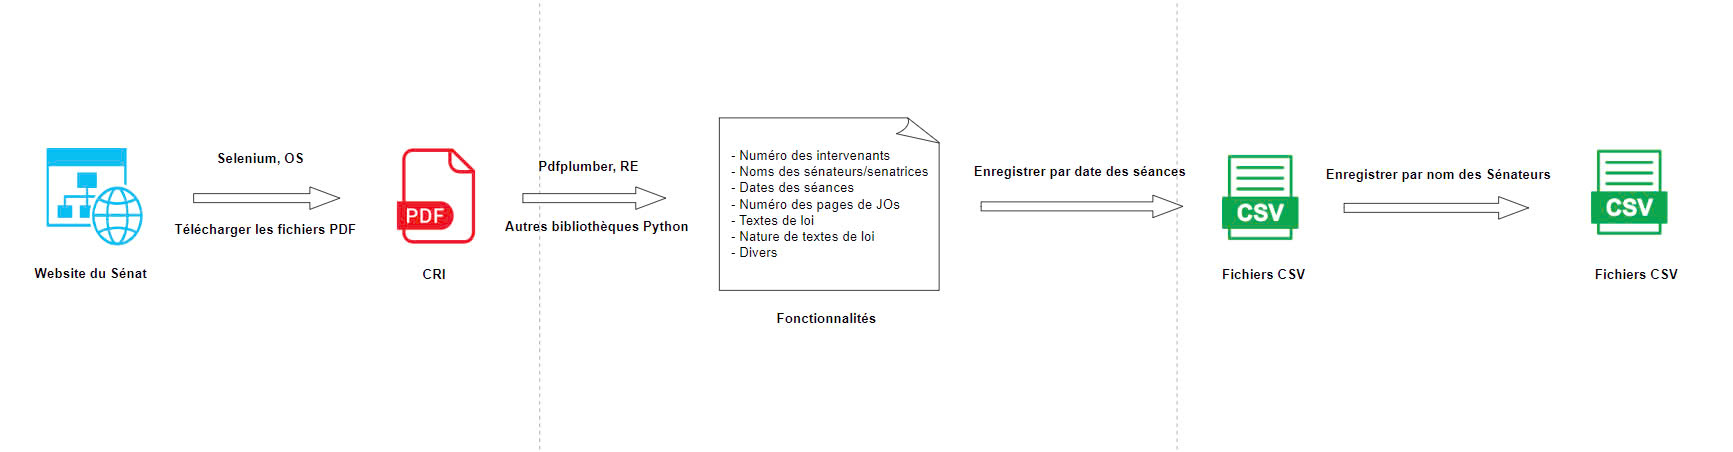
\includegraphics[width=\linewidth]{images/schemas les etapes de travail.jpg} % Đặt đường dẫn đúng tới ảnh của bạn
    \caption{Schéma des étapes de travail}
    \label{fig:schema_travail}
\end{figure}

\subsection{Explication du script}

Ce processus d'automatisation est conçu pour collecter tous les journaux officiels (JO) de l'année 2022 sur le site du Sénat français. Le script utilise l'outil \gls{selenium} pour automatiser la navigation et le téléchargement des fichiers \gls{PDF} à partir du site suivant : \url{https://www.senat.fr/seances/seances.html}. 
Le script identifie les liens vers les fichiers \gls{PDF}, les télécharge à l'aide de la commande \texttt{curl}, et continue le processus jusqu'à ce que tous les fichiers soient récupérés.

\subsubsection{a. Configuration de l'environnement et des bibliothèques}

La première étape consiste à configurer l'environnement et à importer les bibliothèques nécessaires. \gls{selenium} est celle utilisée pour l'automatisation du navigateur, \texttt{os} pour la gestion des fichiers, et \texttt{subprocess} pour exécuter des commandes système telles que \texttt{curl}.

\begin{lstlisting}[language=Python]
from selenium import webdriver
from selenium.webdriver.common.by import By
from selenium.webdriver.common.action_chains import ActionChains
from selenium.webdriver.common.keys import Keys
from selenium.webdriver.support.ui import WebDriverWait
from selenium.webdriver.support import expected_conditions as EC
import time
import os
import subprocess
\end{lstlisting}

\subsubsection{b. Création du dossier pour stocker les fichiers PDF}

Avant de télécharger les fichiers, nous devons créer un dossier pour les stocker. Si ce dossier n'existe pas, il est créé automatiquement.

\begin{lstlisting}[language=Python]
download_dir = "/content/cri_pdf"

if not os.path.exists(download_dir):
    os.makedirs(download_dir)
\end{lstlisting}

\subsubsection{c. Fonction pour télécharger un fichier PDF avec \texttt{curl}}

Cette fonction utilise la commande \texttt{curl} pour télécharger un fichier PDF à partir d'une URL et l'enregistrer dans le dossier spécifié.

\begin{lstlisting}[language=Python]
def download_with_curl(url, download_dir, filename):
    file_path = os.path.join(download_dir, filename)
    subprocess.run(["curl", "-o", file_path, url], check=True)
\end{lstlisting}

\subsubsection{d. Lancement du navigateur et ouverture de la page web}

Ensuite, nous lançons le navigateur Chrome et accédons à la page web du Sénat, où sont répertoriées les séances. Nous attendons que la page se charge avant de procéder.

\begin{lstlisting}[language=Python]
driver = webdriver.Chrome()
driver.get('https://www.senat.fr/seances/seances.html')
time.sleep(5)  # On attend 5 secondes pour que la page se charge
\end{lstlisting}

\subsubsection{e. Utilisation de \texttt{ActionChains} pour faire défiler la page et cliquer sur un bouton}

Pour interagir avec la page, nous utilisons la classe \gls{actionchains} pour simuler des actions comme le défilement et le clic sur des boutons identifiés par leur chemin \gls{xpath} (XML Path Language)

\begin{lstlisting}[language=Python]
actions = ActionChains(driver)

xpath_to_button = '/html/body/main/article/div/div/div/div[1]/div/div[2]/div[1]/div/div/div[3]/h2/button'

while True:
    try:
        WebDriverWait(driver, 10).until(
            EC.element_to_be_clickable((By.XPATH, xpath_to_button))
        ).click()
        time.sleep(3)
\end{lstlisting}

\subsubsection{f. Recherche et traitement des liens vers les fichiers PDF}

Nous identifions une section spécifique de la page contenant des liens vers les fichiers \gls{PDF}. Cette section est identifiée grâce à son chemin \gls{xpath}, et tous les liens sont récupérés.

\begin{lstlisting}[language=Python]
        xpath_to_links_container = '/html/body/main/article/div/div/div/div[1]/div/div[2]/div[1]/div/div/div[3]'
        links_container = WebDriverWait(driver, 10).until(
            EC.presence_of_element_located((By.XPATH, xpath_to_links_container))
        )
        links = links_container.find_elements(By.TAG_NAME, 'a')
\end{lstlisting}

\newpage
\subsubsection{g. Recherche et téléchargement des fichiers PDF}

Le script parcourt ensuite chaque lien trouvé. Pour chaque lien contenant la mention "et au format PDF", l'URL du fichier est récupérée et son contenu téléchargé à l'aide de la fonction \texttt{download\_with\_curl()}.

\begin{lstlisting}[language=Python]
        original_tab = driver.current_window_handle

        for link in links:
            try:
                href = link.get_attribute('href')  # On récupère l'URL du lien
                if href:  # Vérifie si le lien existe
                    driver.get(href)  # Ouvre le lien
                    time.sleep(2)

                    pdf_links = driver.find_elements(By.PARTIAL_LINK_TEXT, "et au format PDF")
                    for pdf_link in pdf_links:
                        try:
                            pdf_href = pdf_link.get_attribute('href')
                            if pdf_href:
                                print(f"URL du fichier PDF: {pdf_href}")

                                file_base = pdf_href.split('/')[-1].split('.')[0]  # Nom du fichier
                                new_filename = f"{file_base}.pdf"  # Nouveau nom du fichier

                                download_with_curl(pdf_href, download_dir, new_filename)

                                time.sleep(5)
\end{lstlisting}

\newpage
\subsubsection{h. Retour à la page précédente et défilement}

Après le téléchargement d'un fichier \gls{PDF}, le script retourne à la page précédente pour traiter les autres liens. En cas d'erreur, il fait défiler la page pour essayer le suivant.

\begin{lstlisting}[language=Python]
                    driver.back()  # Retour à la page précédente
                    time.sleep(2)
            except Exception as e:
                print(f"Impossible de cliquer sur le lien: {e}")

        break
    except Exception as e:
        actions.send_keys(Keys.PAGE_DOWN).perform()
        time.sleep(1)
\end{lstlisting}

\subsubsection{i. Fermeture du navigateur}

Une fois tous les liens traités, le navigateur se ferme pour libérer de la mémoire.

\begin{lstlisting}[language=Python]
driver.quit()
\end{lstlisting}

\section{Étapes d'automatisation de l'extraction}

\subsection{Importation des bibliothèques}

Les lignes de commande ci-dessous importent les bibliothèques nécessaires à la bonne exécution du script : \texttt{os} permet de travailler avec les fichiers et dossiers, \texttt{pdfplumber} est utilisé pour lire et extraire des informations des fichiers PDF, \texttt{pandas} est utilisé pour manipuler les données sous forme de tableaux (DataFrame), et \texttt{shutil} pour copier des fichiers d'un dossier à un autre.

\begin{lstlisting}
import os
import pdfplumber
import pandas as pd
import shutil
\end{lstlisting}
\subsection{2. Fonction \texttt{extract\_bold\_lines\_from\_all\_pages}}
Cette fonction permet d'extraire les lignes de texte en gras de chaque page d'un fichier PDF, \texttt{pdfplumber} est utilisé pour parcourir chaque page et récupérer les mots et groupes de caractères en gras (ce qui est vérifié grâce à la balise \texttt{"Bold"} dans le nom de la police). Si l'un d'eux ne fait pas partie de la liste des termes déjà enregistrés, il est ajouté à cette dernière, puis la boucle continue. 
Dès qu'une ligne complète en gras est détectée, elle est ajoutée à une liste avec le numéro de page correspondant. La fonction renvoie ensuite la liste complète des lignes en gras avec leurs numéros de page individuel.
\begin{lstlisting}
def extract_bold_lines_from_all_pages(pdf_path):
    bold_lines = []
    with pdfplumber.open(pdf_path) as pdf:
        for page_number in range(len(pdf.pages)):
            current_line = ""
            page = pdf.pages[page_number]
            chars = page.chars
            for char in chars:
                if "Bold" in char["fontname"]:
                    current_line += char["text"]
                elif current_line.strip():
                    bold_lines.append((page_number + 1, current_line.strip()))  
                    current_line = ""
            if current_line.strip():
                bold_lines.append((page_number + 1, current_line.strip()))  
    return bold_lines
\end{lstlisting}
\newpage
\subsection{Fonction \texttt{extract\_honorifics}}
Cette fonction extrait les noms des intervenants en fonction de certains préfixes spécifiques (comme \texttt{"Mme le"}, \texttt{"M. le"}, etc.). Elle parcourt les lignes en gras extraites précédemment et recherche ces préfixes. 
Lorsqu'un nom d'intervenant est trouvé, il est enregistré avec le numéro de page correspondant. La fonction retourne ensuite une liste des noms d'intervenants et des numéros de pages.
\begin{lstlisting}
def extract_honorifics(bold_lines):
    honorific_prefixes = ['Mme le', 'Mme la', 'M. le', 'M.', 'Mme']
    extracted_honorifics = []
    page_values = {}
    for page_number, text in bold_lines:
        if text.isdigit():
            page_values[page_number] = text
    for page_number, text in bold_lines:
        for prefix in honorific_prefixes:
            if prefix in text:
                start_index = text.find(prefix)
                end_index = start_index + len(prefix) 
                for i in range(end_index, len(text)):
                    if text[i] in ['.', ',']:
                        end_index = i + 1
                        break
                page_value = page_values.get(page_number, "")
                extracted_honorifics.append((text[start_index:end_index].strip(), page_value))
                break
    return extracted_honorifics
\end{lstlisting}

\newpage
\subsection{Fonction \texttt{process\_pdf\_file}}
Cette section traite chaque fichier \gls{PDF} dans le répertoire spécifié, en extrait les informations avec les fonctions ci-dessus, puis exporte les résultats dans des fichiers \gls{csv} qui sont enregistrés dans un dossier de sortie. La date est extraite du nom du fichier \gls{PDF}, puis formatée afin d'être ajoutée dans le tableau des résultats.
\begin{lstlisting}

def process_pdf_file(pdf_path, date):
    bold_lines = extract_bold_lines_from_all_pages(pdf_path)
    honorifics = extract_honorifics(bold_lines)
    df = pd.DataFrame(honorifics, columns=['Nom_intervenants', 'Num_page'])
    if not df.empty:
        first_president_row = df[(df['Nom_intervenants'] == 'Mme la présidente.') |
                                 (df['Nom_intervenants'] == 'Mme le présidente.') |
                                 (df['Nom_intervenants'] == 'M. le président.') |
                                 (df['Nom_intervenants'] == 'Mme le président.') |
                                 (df['Nom_intervenants'] == 'Mme la président.')].index[0]
        df = df[first_president_row:]
        df['Numero'] = range(1, len(df) + 1)
        df['Date_seances'] = date
        df = df[['Numero', 'Nom_intervenants', 'Date_seances', 'Num_page']]
    return df
\end{verbatim}

Cette fonction prend en entrée un fichier PDF et une date. Elle utilise les fonctions précédentes pour extraire les lignes en gras et les noms des intervenants. Ensuite, elle filtre les noms des intervenants à partir du premier président identifié dans la séance. 
Le résultat est sauvegardé sous forme de tableau avec un numéro d'ordre, le nom de l'intervenant, la date de la séance et le numéro de page.

\subsection{5. Boucle de traitement des fichiers PDF}
\begin{verbatim}
data_dir = "/content/cri_pdf"
output_dir = "/content/compte_intervenants_et_pages"
os.makedirs(output_dir, exist_ok=True)
pdf_files = [f for f in os.listdir(data_dir) if f.endswith('.pdf')]
french_months = ["janvier", "février", "mars", "avril", "mai", "juin", "juillet", "août", "septembre", "octobre", "novembre", "décembre"]
for pdf_file in pdf_files:
    pdf_path = os.path.join(data_dir, pdf_file)
    filename = os.path.splitext(pdf_file)[0]
    year, month, day = filename[1:5], filename[5:7], filename[7:9]
    month_name = french_months[int(month) - 1]
    date = f"{day} {month_name} {year}"
    df = process_pdf_file(pdf_path, date)
    if not df.empty:
        csv_file_name = f"{filename}.csv"
        csv_file_path = os.path.join(output_dir, csv_file_name)
        df.to_csv(csv_file_path, index=False, encoding='utf-8-sig')
\end{lstlisting}
\subsection{Filtrage des noms et copie des fichiers}
Cette partie filtre les fichiers \gls{csv} basés sur une liste de noms d'intervenants prédéfinis et copie les fichiers correspondants dans un autre répertoire. Elle utilise \texttt{shutil.copy2} pour copier chaque fichier tout en préservant ses métadonnées.
\begin{lstlisting}
import shutil
source_folder = 'D:/document/stage/Output'
destination_folder = 'D:/document/stage/Output/filter'
os.makedirs(destination_folder, exist_ok=True)
formatted_names = [...]  # Liste des noms formatés
for filename in os.listdir(source_folder):
    if filename.endswith('.csv'):
        file_name_without_extension = os.path.splitext(filename)[0]
        if file_name_without_extension in formatted_names:
            source_file_path = os.path.join(source_folder, filename)
            destination_file_path = os.path.join(destination_folder, filename)
            shutil.copy2(source_file_path, destination_file_path)
            print(f"File copied: {filename}")
\end{lstlisting}
\subsection{Extraction de sujet et des textes de loi}

\subsubsection{Suppression des termes indésirables}

La première étape consiste à définir une fonction appelée \texttt{remove\_unwanted\_terms()} qui permet de supprimer certains termes indésirables qui apparaissent fréquemment dans le fichier \gls{PDF} mais qui ne sont pas pertinents pour l'extraction des titres. Ces termes incluent des phrases comme "Mme la présidente" ou "M. le président", qui sont souvent répétitifs mais ne fournissent pas d'information utile pour atteindre notre objectif. 

Cette fonction parcourt chaque ligne de texte et remplace les termes indésirables par une chaîne vide, puis renvoie la ligne de texte ainsi nettoyée.

\begin{lstlisting}[language=Python]
def remove_unwanted_terms(text):
    unwanted_terms = [
        'Mme la présidente.',
        'Mme le présidente.',
        'M. le président.',
        'Mme le président.',
        'Mme la président.'
    ]
    for term in unwanted_terms:
        text = text.replace(term, '')
    return text.strip()
\end{lstlisting}
Dans cet exemple, chaque terme indésirable contenu dans le texte est remplacé par une chaîne vide. La fonction \texttt{strip()} est utilisée pour supprimer les espaces en trop après le nettoyage. Cela garantit que les phrases indésirables ne soient plus présentes dans le résultat final.

\subsection{Extraction des titres et du texte}

La fonction principale \texttt{extract\_Titre\_Texte()} est utilisée pour analyser le contenu du fichier \gls{PDF}, page par page, et extraire les sections pertinentes. Elle se concentre principalement sur l'extraction des parties du texte qui sont en gras (ce qui correspond généralement aux titres) ainsi que des sections contenant certains mots-clés, tels que "Article", "Après l’article", ou "Avant l’article", qui sont les indicateurs de sections importantes du document.

\subsubsection{Ouverture du fichier PDF et lecture des caractères}

La fonction commence par ouvrir le fichier \gls{PDF} avec la bibliothèque \texttt{pdfplumber}. Ensuite, elle parcourt chaque page du document et analyse les caractères présents sur chaque ligne pour détecter ceux qui sont en gras. Les caractères en gras sont généralement associés aux titres, c'est pourquoi cette détection est essentielle pour la structuration des données.
\begin{lstlisting}
def extract_Titre_Texte(pdf_path):
    data = []
    expected_number = 1  # Variable pour suivre le numéro attendu
    with pdfplumber.open(pdf_path) as pdf:
        for page_number in range(len(pdf.pages)):
            current_line = ""
            page = pdf.pages[page_number]
            chars = page.chars  # 'chars' est un dictionnaire des caractères

            for char in chars:
                if "Bold" in char["fontname"]:  # Si le caractère est en gras
                    current_line += char["text"]  # Ajoute le texte en gras
                elif current_line.strip():  # Si la ligne est terminée
                    match = re.match(r"(\d+)\s+([A-Za-zÀ-Ýa-zà-ý\s:’.,;?!()\[\]«»\-]*)(?:\s*(Mme la présidente\.|Mme le présidente\.|M\. le président\.|Mme le président\.|Mme la président\.))?$", current_line.strip())
                    if match and int(match.group(1)) == expected_number:
                        expected_number += 1  # Incrémenter le numéro attendu
                        title_text = f"{match.group(2).strip()}"
                        data.append((page_number + 1, current_line.strip(), title_text, ""))
                    else:
                        data.append((page_number + 1, current_line.strip(), None, ""))
                    current_line = ""
\end{lstlisting}
Dans cet extrait de code, la fonction vérifie chaque caractère pour déterminer s'il est en gras (reconnaissable grâce à l'attribut \texttt{"Bold"} dans le nom de la police). Lorsque des caractères en gras sont détectés, ils sont concaténés dans une chaîne de texte qui est ensuite traitée comme un titre potentiel.

\subsubsection{Traitement des fins de pages et suppression des termes indésirables}

À la fin de chaque page, il est possible que certaines informations non pertinentes, comme des numéros de page, apparaissent. La fonction \texttt{remove\_unwanted\_terms()} est ensuite appelée pour supprimer ces éléments indésirables dans les titres avant de finaliser les données extraites.

\begin{lstlisting}[language=Python]
# Supprimer les mots non souhaités à la fin du texte (Mme la présidente) du TITRE
for i in range(len(data)):
    if data[i][2] is not None:
        data[i] = (data[i][0], data[i][1], remove_unwanted_terms(data[i][2]), data[i][3])
\end{lstlisting}
Cette boucle parcourt les données extraites, vérifie si le titre contient l'un des termes indésirables, et applique la fonction \texttt{remove\_unwanted\_terms()} pour nettoyer les résultats.

\subsubsection{Remplissage des valeurs manquantes et détection du texte}

Une fois les titres extraits et nettoyés, les valeurs manquantes sont comblées. Si une ligne n'a pas de titre explicite, le titre de la ligne précédente est utilisé. De même, les sections contenant les mots-clés comme "Article", "Après l’article", ou "Avant l’article" sont identifiées et ajoutées à la colonne \textbf{Texte}.
\begin{lstlisting}
# Remplacer les valeurs 'none' ou vides par celles du Titre précédent
last_titre_text = None
for i in range(len(data)):
    if data[i][2] is not None:
        last_titre_text = data[i][2]
    elif last_titre_text is not None:
        data[i] = (data[i][0], data[i][1], last_titre_text, data[i][3])

# Si les valeurs en gras contiennent des termes tels que : Après l’article, Article, Avant l’article, les ajouter à la liste (thème)
for i in range(len(data)):
    if data[i][1] and ("Après l’article" in data[i][1] or "Article" in data[i][1] or "Avant l’article" in data[i][1]):
        data[i] = (data[i][0], data[i][1], data[i][2], data[i][1])
\end{lstlisting}

Dans ce processus, la fonction remplit les valeurs manquantes en utilisant les titres précédents pour garantir qu'aucune ligne ne soit laissée vide. Ensuite, elle identifie les sections textuelles pertinentes à l'aide de mots-clés spécifiques.

\subsubsection{Fonction \texttt{extract\_topic} pour extraire la nature des articles de loi}

La fonction \texttt{extract\_topic()} est utilisée pour extraire les informations relatives aux thèmes à partir d’un fichier \gls{PDF}. Ces thèmes pertinents incluent des zones de texte en majuscules mais non en gras, et qui contiennes, par exemple, les termes "PROPOSITION DE LOI" ou "PROJET DE LOI". La variable \texttt{topic\_lines} est quant à elle appelée comme liste vide dont le rôle et de lister ces lignes de texte correspondantes aux thèmes identifiés.

\begin{lstlisting}[language=Python]
def extract_topic(pdf_path, data):
    topic_lines = []
\end{lstlisting}

Ensuite, la fonction utilise \texttt{\gls{pdfplumber}} pour ouvrir et lire le contenu du fichier \gls{PDF}. Ce dernier est ouvert à l'aide de \texttt{pdfplumber.open()}, et chaque page du fichier est parcourue via une boucle \texttt{for}. Les caractères sur chaque page sont extraits.

\begin{lstlisting}[language=Python]
with pdfplumber.open(pdf_path) as pdf:
    for page_number in range(len(pdf.pages)):
        current_line = ""
        page = pdf.pages[page_number]
        chars = page.chars
\end{lstlisting}

Le code vérifie chaque caractère pour déterminer s'il est en gras ou non (en se basant sur l'attribut \texttt{Bold} dans \texttt{fontname}). Si le caractère n'est pas en gras, il est ajouté à la chaîne \texttt{current\_line}.

\begin{lstlisting}[language=Python]
for char in chars:
    if "Bold" not in char["fontname"]:
        current_line += char["text"]
\end{lstlisting}

Une fois que les caractères non en gras sont collectés, le code vérifie si la chaîne \texttt{current\_line} contient l'une des expressions "PROPOSITION DE LOI" ou "PROJET DE LOI". Si l'une des expressions est trouvée, la ligne de texte actuelle, ainsi que le numéro de page, sont ajoutés à la liste \texttt{topic\_lines}.

\begin{lstlisting}[language=Python]
if "PROPOSITION DE LOI" in current_line or "PROJET DE LOI" in current_line:
    topic_lines.append((page_number + 1, current_line))
\end{lstlisting}

\newpage
Après avoir collecté les lignes de texte relatives au thème, le code utilise des expressions régulières (\gls{regex}) pour rechercher et extraire avec précision les parties du texte contenant "PROPOSITION DE LOI" ou "PROJET DE LOI".

\begin{lstlisting}[language=Python]
pattern_proposition = r'\b[A-ZÀ-Ý\s\.,;’!?()_-]*PROPOSITION DE LOI[A-ZÀ-Ý\s\.,;’!?()_-]*\b'
matches_proposition = re.findall(pattern_proposition, text, re.DOTALL)

pattern_projet = r'\b[A-ZÀ-Ý\s\.,;’!?()_-]*PROJET DE LOI[A-ZÀ-Ý\s\.,;’!?()_-]*\b'
matches_projet = re.findall(pattern_projet, text, re.DOTALL)
\end{lstlisting}
Les modèles d'expressions régulières \texttt{pattern\_proposition} et \texttt{pattern\_projet} recherchent les expressions "PROPOSITION DE LOI" et "PROJET DE LOI" dans le texte, avec des caractères en majuscules, espaces, ponctuations avant et après. 

Les résultats extraits par les \gls{regex} sont ensuite nettoyés. Les espaces multiples sont remplacés par un seul, et les caractères spéciaux au début et à la fin de la chaîne sont supprimés. Le processus fonctionne de la sorte : tout d'abord, les espaces multiples dans la chaîne \texttt{match} sont remplacés par un seul espace via la fonction \texttt{re.sub}. Ensuite, les caractères indésirables au début et à la fin de la chaîne sont retirés automatiquement par la fonction.
\begin{lstlisting}[language=Python]
cleaned_match = re.sub(r'\s+', ' ', match.strip())
cleaned_match = re.sub(r'^[\s\.,;’!?()_-]+|[\s\.,;’!?()_-]+$', '', cleaned_match)
\end{lstlisting}
Le code vérifie ensuite si le dernier mot de la chaîne est trop court (moins de 2 caractères), si c’est le cas, il est supprimé. Cela permet de s'assurer que les mots incomplets ou trop courts ne sont pas conservés dans le résultat final.
\begin{lstlisting}[language=Python]
while words and len(words[-1]) < 2:
    words.pop()
cleaned_match = ' '.join(words)
\end{lstlisting}
Enfin, le thème est ajouté aux données d'origine (\texttt{data}) en fonction du numéro de page. Si une page a un thème, il est ajouté à la cinquième colonne de chaque ligne.
\begin{lstlisting}[language=Python]
for i in range(len(data)):
    page_number = data[i][0]   
    if page_number in theme_lines:
        data[i] = (data[i][0], data[i][1], data[i][2], data[i][3], theme_lines[page_number])
\end{lstlisting}
Si une ligne ne contient pas de thème, le code remplace cette valeur par le thème de la page précédente. Cela garantit que toutes les lignes ont un thème, sans laisser de colonne vide.
\begin{lstlisting}
last_topic_text = ""
for i in range(len(data)):
    if len(data[i]) > 4 and data[i][4] != "":
        last_topic_text = data[i][4]
    else:
        data[i] = (data[i][0], data[i][1], data[i][2], data[i][3], last_topic_text)
\end{lstlisting}
Enfin, les données traitées, avec les thèmes associés à chaque page du fichier \gls{PDF}, sont retournées par la fonction.
\begin{lstlisting}[language=Python]
return data
\end{lstlisting}
Ce processus permet d’identifier et d’extraire efficacement les informations liées à des propositions ou projets de loi à partir de fichiers \gls{PDF} complexes, en les organisant de manière structurée pour une utilisation ultérieure.


\section{Évaluation des performances}

\subsection{Qualité de l’éxtraction}


\begin{table}[ht!]
\centering
\begin{tabular}{|c|p{8cm}|}
\hline
\textbf{Nom de colonne} & \textbf{Description} \\
\hline
Numero & Numéro d'intervenant \\
\hline
Date\_seances & Date des séances publiques \\
\hline
Num\_page & Numéro des pages du \textit{Journal Officiel} \\
\hline
Titre & Divers, sujet général de contenu de discussion \\
\hline
Texte & L'article de loi discuté \\
\hline
Thème & Nature du texte des articles de loi \\
\hline
\end{tabular}
\caption{Description des colonnes du fichier CSV}
\label{table:description_csv}
\end{table}


\subsubsection{Partie 1: Numérotation des intervenants, Nom des Sénateurs, Numéro de pages}

Après plusieurs ajustements du script d'extraction automatique, notamment l'optimisation des algorithmes de reconnaissance de motifs et l'amélioration de la gestion des lignes en gras pour identifier les intervenants, les résultats obtenus ont montré une précision considérablement améliorée. De plus, lorsque l'extraction automatisée est comparée à l'entrée manuelle, la méthode automatisée produit de meilleurs résultats et se montre plus rapide rapide, avec une réduction significative des erreurs.

Les chaînes d'extraction ajustées ont fonctionné de manière efficace en isolant correctement les noms des intervenants, les numéros de page, et d'autres métadonnées critiques des documents \gls{PDF}. En particulier, les améliorations apportées au traitement des textes en gras ont permis de capturer les noms et les numéros d'intervenants avec une précision bien supérieure. En effet, dans les étapes précédentes, certaines erreurs pouvaient apparaître, notamment lorsque plusieurs intervenants étaient affichés sur la même page, ou dans le cas où des titres non pertinents étaient pris en compte. Grâce aux ajustements, ces erreurs ont été corrigées, permettant une identification plus claire et précise des informations pertinentes.
Le résultat est un total de 85 fichier \gls{CSV} correspondant aux 85 sessions de l'année 2022, pour comparer facilement la précision de l'extraction, voici 2 captures d'écran des résultats de test de l'application \gls{Prepub} ainsi que le tableau issu du processus d'automatisation au 22 février 2022 :

\begin{figure}[H]
    \centering
    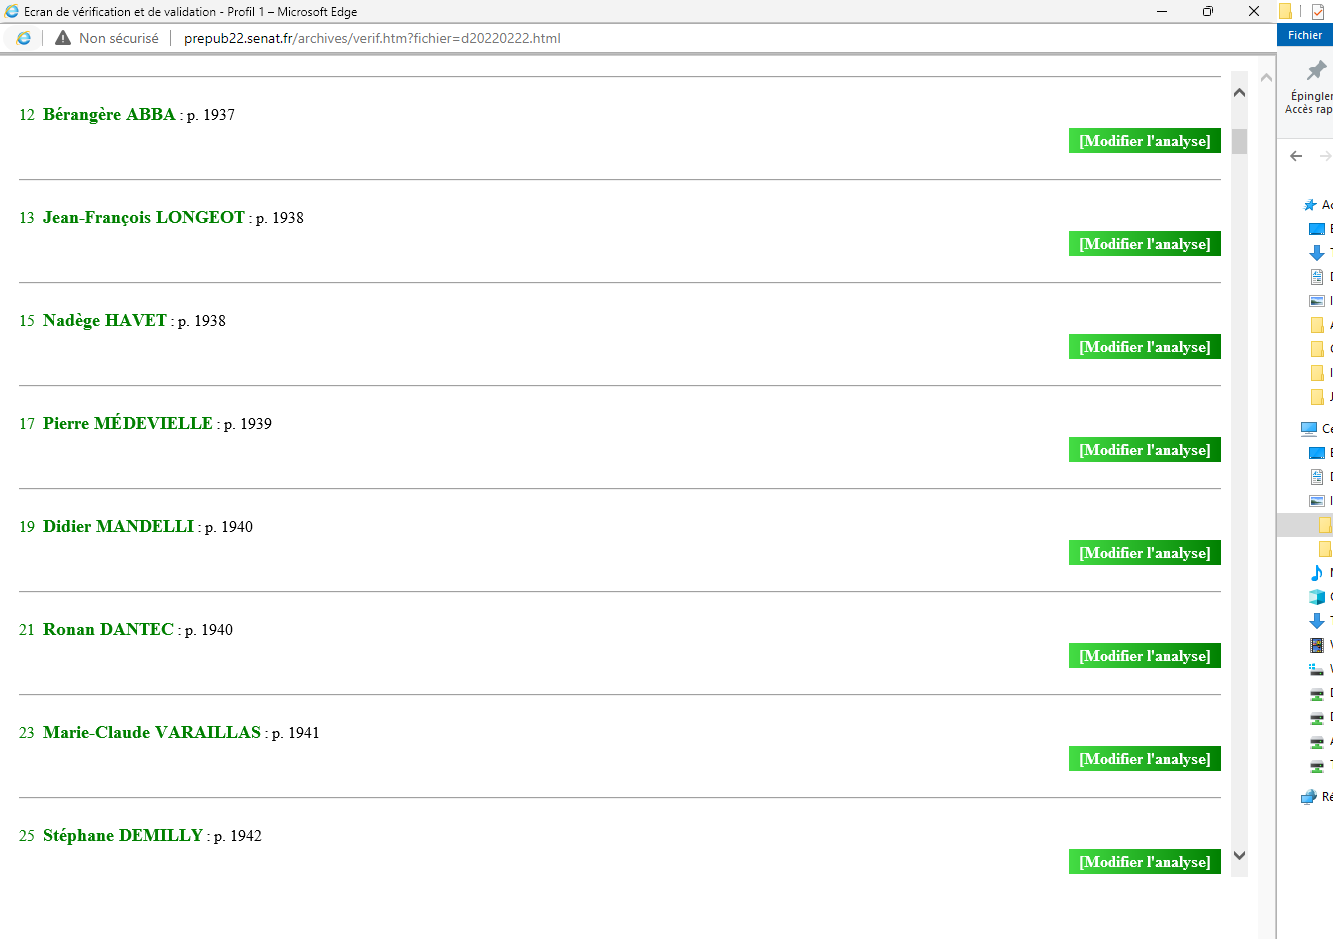
\includegraphics[width=1\textwidth]{images/check 4.PNG}
    \caption{Capture d'écran de vérification et de validation d'application archives Prépub}
\end{figure}

\begin{figure}[H]
    \centering
    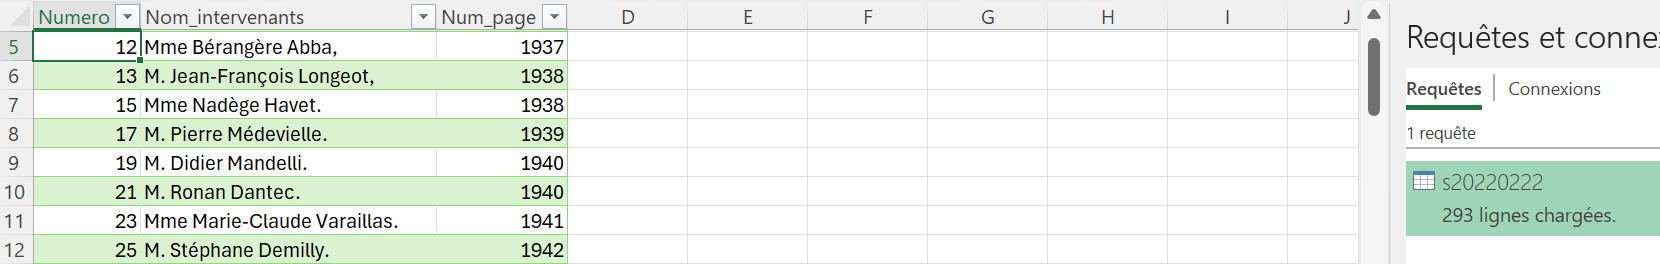
\includegraphics[width=1\textwidth]{images/verifie4.png}
    \caption{Capture d'écran de tableaux extrait}
\end{figure}

Nous pouvons voir que les numéros des intervenants se correspondent parfaitement sur les deux résultats : 12, 13, 15, 17, 19, 21, 23, 25... .\\
Concernant le nom des intervenants, ils sont également identiques, cependant, sur les photos du site, ces derniers sont écrits en majuscules pour les noms de famille (par exemple Bérangère ABBA au lieu de Mme Bérangère Abba) ; de même, les titres « Mme » et « M ». n'apparaissent pas dans la capture d'écran du site Web, car seuls le prénom et nom de famille sont affichés. Nous pouvons cependant, grâce à un script, exécuter une commande afin de nettoyer cette mise en forme et mettre tous les noms de famille des orateurs en majuscule. .\\
Enfin, les numéros de page se correspondent également parfaitement : 1937, 1938, 1939, 1940, 1941, 1942. De plus, la date de la session est extraite du nom du fichier de la session au format saaaammdd (s = séance; aaaa = année; mm= mois, dd=date), les résultats seront donc précis et correspondront aux autres informations extraites de la session du jour.

\newpage
\subsubsection{Partie 2: Textes de loi, Nature de textes, Divers}

Prenons l'exemple de la table des matières de la Sénatrice Mélanie Vogel.

\begin{figure}[H]
    \centering
    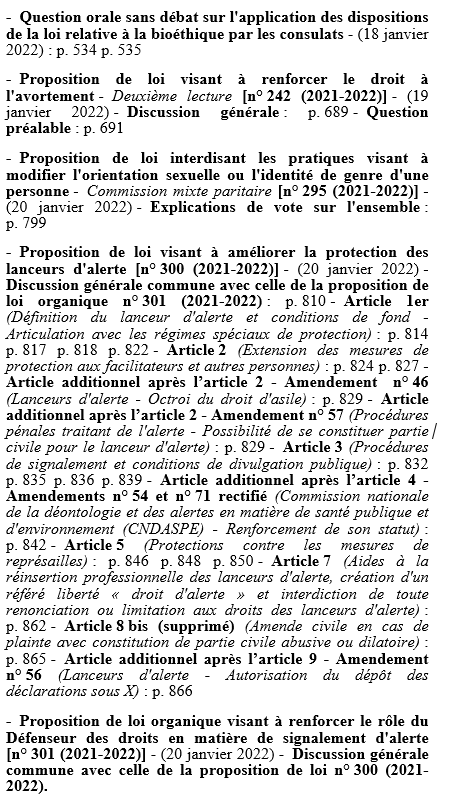
\includegraphics[width=0.7\textwidth]{images/check5table.png}
    \caption{Capture d'écran de table du Sénat de Mme Mélanie Vogel 2022}
\end{figure}

\begin{figure}[H]
    \centering
    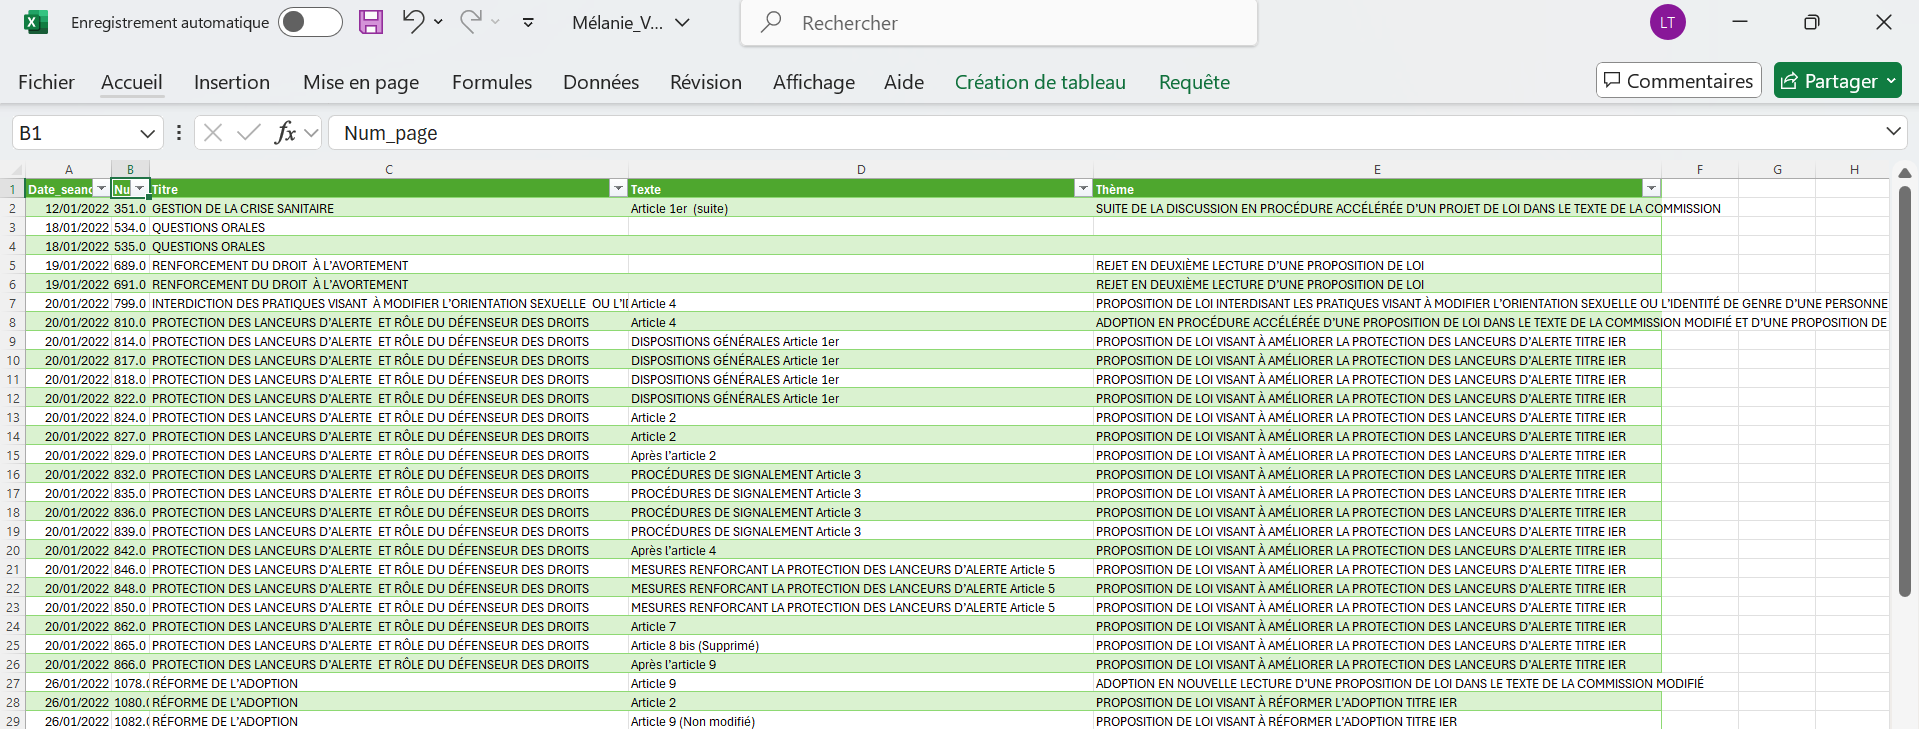
\includegraphics[angle=90, width=0.6\textwidth]{images/Capture d'écran 2024-09-28 034312.png}
    \caption{Capture d'écran de tableaux extrait automatique}
\end{figure}

\paragraph{} On note la présence de beaucoup d'informations détaillées dans les tables du Sénat, à la fois complètes et précise, incluant des éléments comme : les sujets, les dates, les numéros de page, les types de documents, et des contenus supplémentaires comme les questions, les discussions générales, etc. En ce qui concerne le tableau extrait automatiquement, il manque des informations sur les thèmes, et la colonne du texte retire parfois des informations non pertinentes. Cela complique la recherche d'informations dans le tableau lorsqu'il est nécessaire de les comparer avec les documents originaux. Bien que l'extraction automatique ait permis de récupérer une partie des titres et des articles avec précision, les informations complémentaires importantes ne sont pas encore suffisantes pour en faire une table des matières complète.

En termes de précision de la structure et de mise en forme dans la table des matières du Sénat, les éléments sont bien formatés, avec des espaces et des signes clairement définis. Cependant, dans le tableau automatisé, bien que le contenu principal soit extrait, la mise en forme n'est pas toujours normalisée. Par exemple, certaines parties extraites sont répétées plusieurs fois, avec des espaces ou des ponctuations inutiles, ce qui entraîne une confusion au niveau de l’apparence. Les symboles spéciaux, comme les guillemets ou les informations sur l'état de modification (par exemple "Article 8 bis (supprimé)"), ne sont pas traités de manière cohérente. En outre, en termes d'exhaustivité du contenu, certains articles peuvent ne pas être complètement extraits ou il peut en manquer certaines parties, en particulier lorsque les titres sont trop longs ou possèdent une structure complexe. Cette situation crée un écart dans l'exhaustivité des informations par rapport à la table des matières réelle. Dans cette dernière, des informations telles que "Proposition de loi n° 300", "Adoption en nouvelle lecture", "Débat sur..." sont entièrement et précisément notées. Pour expliquer cette extraction partielle du contenu, nous pouvons prendre l'exemple de la ligne "Question orale sans débat sur l'application des dispositions de la loi relative à la bioéthique par les consulats" qui, dans le tableau automatisé, n'a extrait que "QUESTIONS ORALES". La partie "sur l'application des dispositions de la loi relative à la bioéthique par les consulats" n'apparaît pas dans le PDF du JO, car cette partie est ajoutée manuellement, et n'est donc pas disponible pour l'extraction automatique.

Nous constatons d'ailleurs que les tables des matières du Sénat ne répètent généralement pas plusieurs fois les mêmes articles ou les informations redondantes. Cependant, dans le tableau automatisé, l'extraction automatique est encore trop brute et peut parfois conduire à des informations répétées, avec des contenus superposés, par exemple, "Proposition de loi visant à améliorer la protection des lanceurs d'alerte" qui apparaît à plusieurs reprises.


\subsection{Limites}

En ce qui concerne la numérotation des intervenants, les scripts sont configurés pour compter les éléments en gras au début des lignes, comme "M." et "Mme" suivis du nom propre et d'un point "." ou d'une virgule ",". Cependant, dans certains cas exceptionnels, comme illustré ci-dessous, le début de ligne en gras ne commence pas par "M." ou "Mme", mais par la phrase \textit{"Plusieurs sénateurs du groupe Les Républicains. Il n’a pas répondu !"}. Cela signifie que ces cas particuliers ne sont pas pris en compte dans le comptage automatique. Bien que cela n'affecte ni le numéro de page ni le contenu de la table des matières, cela peut créer un décalage dans le décompte des intervenants par rapport à la numérotation affichée dans \gls{Prepub}. 

Dans ces cas rares, il est possible de modifier le script pour corriger ce problème de manière spécifique. Cependant, il est important de noter qu'aucun outil d'automatisation ne peut garantir une précision absolue, et que, par conséquent, des vérifications manuelles et des corrections ponctuelles sont parfois inévitables.

\begin{figure}[H]
    \centering
    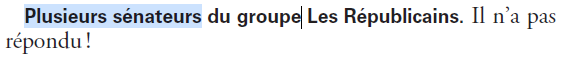
\includegraphics[width=0.7\textwidth]{images/Capture d'écran 2024-09-28 041223.png}
    \caption{Capture d'écran d'un JO}
\end{figure}

En outre, en ce qui concerne l'extraction des thèmes, l'automatisation présente encore plusieurs aspects à améliorer. L'ajout d'informations telles que les numéros de page, les dates et d'autres détails supplémentaires est essentiel pour que l'automatisation puisse atteindre une qualité équivalente à celle des tables des matières du Sénat. Il faudra également prévoir des étapes supplémentaires de traitement pour éliminer les doublons et les données superflues, afin de garantir que les données extraites soient nettes et précises. Pour les parties contenant de nombreux symboles ou des informations supplémentaires, il sera également indispensable d'améliorer la capacité de reconnaissance et de traitement de ces sections afin d'obtenir des résultats d'extraction encore plus précis.
\newpage
\section{Facilitation de la saisie d’information}

Même s'il est actuellement impossible d'automatiser complètement la création des Tables du Sénat, nous pouvons tout de même tirer parti de certaines colonnes du fichier \gls{csv}, notamment le numéro d'intervention, le nom de l'intervenant, et le numéro de page. Ces informations peuvent être intégrées avec un haut niveau de précision dans un fichier \gls{XML}, fichier qui pourra ensuite être chargé dans l'application \gls{Prepub} pour valider les comptes rendus des séances ou pourra servir à générer des tables des matières dans des formats tels que Word à travers la Direction d'Information du Sénat.
Le processus de conversion des données d'un fichier \gls{csv}vers un format \gls{XML} repose sur plusieurs étapes importantes. Tout d'abord, l'utilisation de la bibliothèque `\gls{pandas}` qui permet de lire le fichier CSV et d'organiser ses données sous forme de DataFrame. Le tableau ainsi généré contient des colonnes telles que "Num\_page", "Numero" et "Nom\_intervenants", représentant respectivement le numéro de page, le numéro d'intervention et le nom de l'intervenant. Une fois ces données organisées, la transformation en \gls{XML} nécessite la création de balises spécifiques. Par exemple, une balise `<cri:intervenant>` est utilisée pour encapsuler les informations liées à chaque intervenant. À l'intérieur de cette balise, on insère des attributs comme `nom` pour le nom de l'intervenant, `id` pour le numéro d'intervention et `analyse` pour le numéro de page associé. \footcite{askpython_csv_to_xml}

Ensuite, chaque ligne du DataFrame est parcourue, et pour chaque enregistrement, une nouvelle balise \gls{XML} est générée avec les informations correspondantes. Ces balises sont ensuite organisées dans une structure \gls{XML} hiérarchique où les éléments sont imbriqués selon leur relation avec les autres données. La conversion est réalisée grâce à la méthode `\gls{elementtree}` de la bibliothèque `xml.etree.ElementTree`, qui permet d'écrire les balises générées dans un fichier \gls{XML}.

Ce processus offre de nombreux avantages, notamment la possibilité d'utiliser ces données dans des systèmes qui nécessitent un format standardisé tel que \gls{XML} Cela permet également une interopérabilité accrue avec d'autres outils ou systèmes d'archivage. Une fois les données converties, elles peuvent être intégrées dans des bases de données ou utilisées pour des analyses ultérieures, tout en garantissant un format cohérent et lisible par les machines.


\begin{table}[ht]
    \centering
    \begin{adjustbox}{max width=\textwidth}
    \begin{tabular}{|l|l|p{8cm}|} % Adjust the width of the third column
        \hline
        \textbf{Type d'annotations} & \textbf{Balise XML/Attribut résultant} & \textbf{Copier à la main le XML correspondant} \\ \hline
        \textbf{Nom d’intervenants} & \verb|<cri:intervenant>| \verb|nom=| & \lstinline|<cri:intervenant id="int_11" parid="par_40" mat="12028B" nom="Marie-Arlette CARLOTTI" civ="Mme" qua="" type="1" analyse="p. 4170" checked="O">| \\ \hline
        \textbf{Numéro d'intervention} & \verb|<cri:intervenant>| \verb|id=| & \lstinline|<cri:intervenant id="int_11" parid="par_40" mat="12028B" nom="Marie-Arlette CARLOTTI" civ="Mme" qua="" type="1" analyse="p. 4170" checked="O">| \\ \hline
        \textbf{Numéro de page} & \verb|<cri:intervenant>| \verb|analyse=| & \lstinline|<cri:intervenant id="int_11" parid="par_40" mat="12028B" nom="Marie-Arlette CARLOTTI" civ="Mme" qua="" type="1" analyse="p. 4170" checked="O">| \\ \hline
        \textbf{Article} & \verb|<cri:mentionarticle>| \verb|num=| \verb|info=| & \lstinline|<cri:mentionarticle parid="par_2018" id="debut_detail_loi_22" type="1" num="Article�13" info="Soumission des terminaux méthaniers flottants à un régime administratif propre"><a name="R13"> </a><p class="mention_article" id="par_2018">Article&#160;13</p></cri:mentionarticle>| \\ \hline
    \end{tabular}
    \end{adjustbox}
    \caption{Table des annotations et balises XML correspondantes}
\end{table}





